\documentclass{article}[11pt]
\textheight 8.5in
\usepackage{graphicx}
\usepackage{float}%for forcing position of figs
\usepackage{hyperref}
\usepackage{amsmath}
\usepackage{amssymb}

\begin{document}
\begin{center}
Siddharthan Rajasekaran\\
Week of 3/20/2017 - 3/27/2017
\end{center}

\section{Summary of Discussions}
In this report, we will show the results of EM algorithm applied to a multi-agent IRL using demonstrations collected from toy example. 

\section{Setup}
We consider a $5 \times 5$ grid with two agents. Agent-1's policy is to randomly pick from [``up'', ``right"] and that of agent-2 is to pick from [``down'', ``left"] (with uniform random distribution for both agents). Hence we can expect that agent-1 gets a high reward at the top-right and that agent-2 gets a high reward at the bottom-left of the gridworld. We generate, starting at random states, $100$ trajectories from agent-1 and $200$ trajectories from agent-2 and append them into one list of demonstrations. The length of each trajectory is $50$. The discount factor of the MDP is $0.9$

\section{Results}
We will revisit some of the terms in the previous report to better interpret the results. 

Remember that $\beta_{ij}$ is the probability $P(c_j|D_i)$ and $\Psi(c_j)$ is the prior probability of class $c_j$. We would want, at convergence, $\Psi(c_1) = 0.33$ and $\Psi(c_2) = 0.67$ (or) $\Psi(c_1) = 0.67$ and $\Psi(c_2) = 0.33$ (both are equivalent since the ordering of the class can be interchanged)

\begin{align}
\label{def_beta}
\beta_{ij}^{(t)} &= \frac{P(\mathcal{D}_i| c_j,\Theta^{(t)},\Psi^{(t)})\Psi^{(t)}(c_{j})}{\sum_k P(\mathcal{D}_i| c_k,\Theta^{(t)},\Psi^{(t)})\Psi^{(t)}(c_{k})}\\
\label{def_unn}
\tilde{\beta}_{ij}^{(t)} &= P(\mathcal{D}_i| c_j,\Theta^{(t)},\Psi^{(t)})\Psi^{(t)}(c_{j})
\end{align} As we expected, the EM algorithm converges, but not at the optimal answer always. For example, we ran the EM algorithm $20$ times on the above experiments and $8$ times the EM converged to a local minima or saddle point with $\Psi(c_1) = 1$ and $\Psi(c_2) = 0$ (or) $\Psi(c_1) = 0$ and $\Psi(c_2) = 1$, while $12$ times it converged to the expected values. We get the following results in these cases, (in the following we use the term confidence metric very loosely)




 \begin{figure}[H]
  \begin{center}
    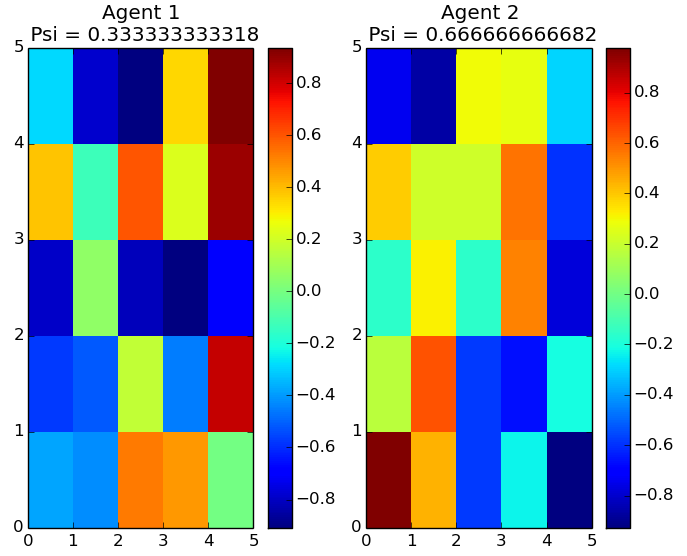
\includegraphics[width=1\linewidth]{images/rewards6}
    \caption{\textbf{Converged to expected value.} Learned reward function for the two agents. We have the expected prior on $\Psi$. Note how the reward function of both the agents are estimated correctly. That is, for agent-1, we have positive rewards in top right and for agent-2 we have them in bottom left.}
    \label{fig:5grid}
  \end{center}
\end{figure}

 \begin{figure}[H]
  \begin{center}
    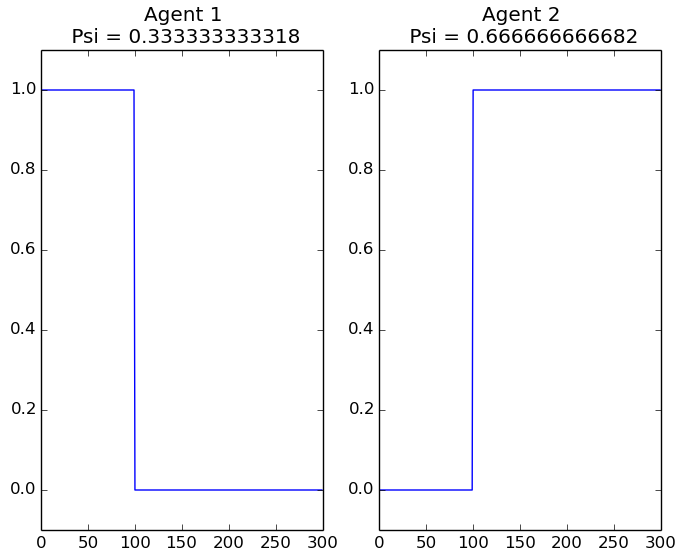
\includegraphics[width=1\linewidth]{images/P(c|D)6}
    \caption{\textbf{Converged to expected value.} $P(c_j|D_i)$ vs $i$ i.e, $\beta_{ij}$ vs index of demonstrations. Note that the first 100 demonstrations are correctly attributed to agent-1 with probability close to $1$}
    \label{fig:5grid}
  \end{center}
\end{figure}

 \begin{figure}[H]
  \begin{center}
    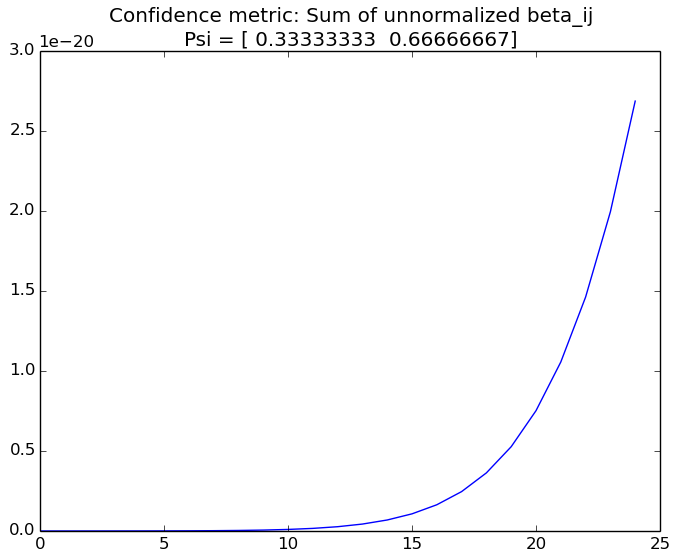
\includegraphics[width=1\linewidth]{images/confidence6}
    \caption{\textbf{Converged to expected value.} Confidence metric: $\sum_{i,j} \tilde{\beta}_{ij}$ vs the number of iterations. Note how this confidence metric increases as we learn better parameters for the model}
    \label{h_c}
  \end{center}
\end{figure}


 \begin{figure}[H]
  \begin{center}
    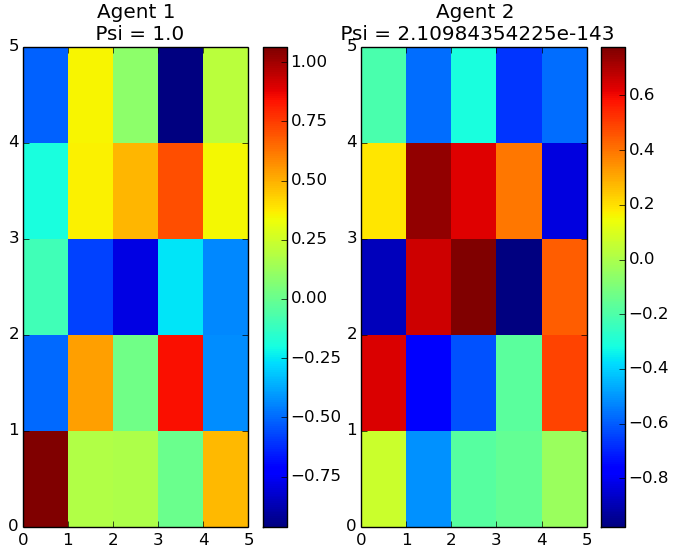
\includegraphics[width=1\linewidth]{images/rewards0}
    \caption{ \textbf{Converged to saddle point.} Learned reward function for the two agents. We have a wrong prior on $\Psi$. However, note that we have learned the correct reward function for agent-1 due to high prior on agent-1}
    \label{fig:5grid}
  \end{center}
\end{figure}

 \begin{figure}[H]
  \begin{center}
    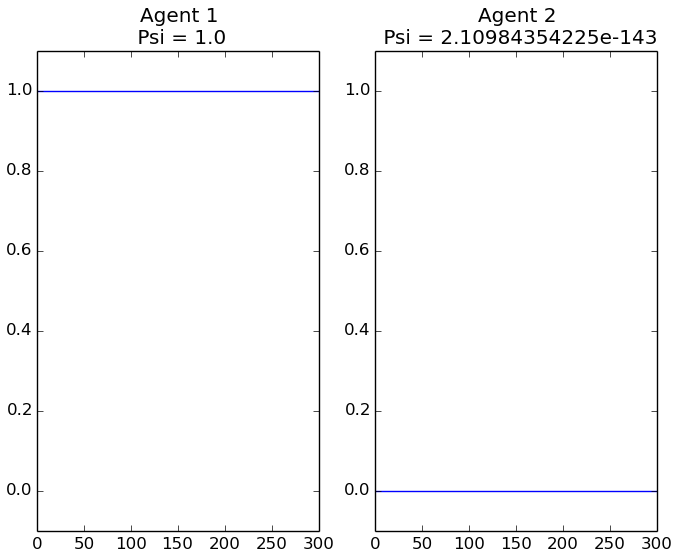
\includegraphics[width=1\linewidth]{images/P(c|D)0}
    \caption{\textbf{Converged to saddle point.} $P(c_j|D_i)$ vs $i$ i.e, $\beta_{ij}$ vs index of demonstrations. Note that all demonstrations are attributed to agent-1.}
    \label{fig:5grid}
  \end{center}
\end{figure}

 \begin{figure}[H]
  \begin{center}
    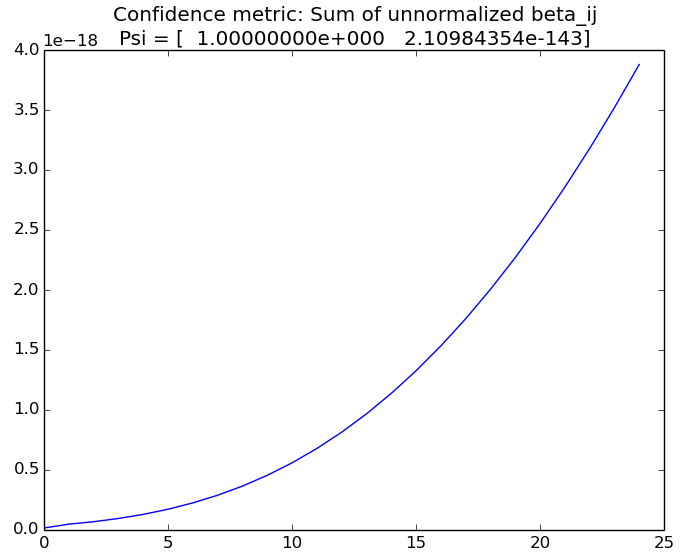
\includegraphics[width=1\linewidth]{images/confidence0}
    \caption{\textbf{Converged to saddle point.} Confidence metric: $\sum_{i,j} \tilde{\beta}_{ij}$ vs the number of iterations. Note how this confidence metric increases as we learn better parameters for the model}
    \label{h_w}
  \end{center}
\end{figure}

\subsection{Problems using fixed number of classes}

\begin{enumerate}
\item Random restarts does solve the problem. But we must have a way to say that $\Psi = [0.33,0.67]$ is better than $\Psi = [1,0]$. I tried to use $\sum_{i,j} \tilde{\beta}_{ij}$ (as an indicator of confidence level) but it seems to not work as shown in the above plots. Note that the metric is of the order $\exp(-20)$ for the correct value of $\Psi$ in Fig. \ref{h_c} and is of the order $\exp(-18)$ in Fig. \ref{h_w} for the wrong values. 
\item Need to test if $\sum_{i,j}P(D_i|c_j)$ can be a better metric.
\end{enumerate}

\subsection{Using Dirichlet Prior}
Using Dirichlet prior for the classes ,$\Psi(c_j)$, solves the problem of getting stuck at local minima for the above toy problem. The generative model is that the class is first sampled from $\Psi(c_j)$, then we sample the trajectory given the reward function of that class. We compute $P(c_j|\mathcal{D}_i)$ directly from 

\begin{align*}
P(c_j|\mathcal{D}_i) = \eta \cdot P(\mathcal{D}_i|c_j)\Psi(c_j)
\end{align*} 

One problem in doing the above is that we would get some non-zero probability for a new class for every demonstration. Hence we would have as many as classes as the demonstrations. This means we would have to solve $n$ different MaxEnt problems at every iteration. Hence the algorithm would scale much poorly with data. One work around for this problem is to re-sample from the distribution  $P(c_j|\mathcal{D}_i)$. This means that classes with lesser probability of occurrence have much less probability of being sampled. This is analogous to the resampling step in particle filter, where we want to maintain the same number of particles but approximate a different distribution. Also, the particles with very small weights (which do not agree with the observations) do not get re sampled.  

\subsection{Racetrack example}
We try to use the same algorithm on yet another toy example. We have a race track as shown in the figure 


\nocite{ziebart2010modeling}
\section{Bibliography}

\bibliographystyle{plain}
\bibliography{bibfile}
\end{document}
